\chapter{Tín hiệu âm thanh, tiếng nói. Thư viện PyAudio}
\ifpdf
    \graphicspath{{Chapter2/Chapter2Figs/PNG/}{Chapter2/Chapter2Figs/PDF/}{Chapter2/Chapter2Figs/}}
\else
    \graphicspath{{Chapter2/Chapter2Figs/EPS/}{Chapter2/Chapter2Figs/}}
\fi

\section{Tổng quan}
\subsection{Tổng quan về âm thanh}
Trong vật lý, âm thanh được định nghĩa là các giao động cơ học lan truyền thông qua các phương tiện truyền dẫn như: không khí, nước, chất rắn,... Các giao động cơ học đó còn được gọi là sóng âm. Sóng âm được tạo ra do có sự biến đổi về áp suất theo thời gian. Vận tốc lan truyền trong không khí của sóng âm vào khoảng 343.2 m/s.

Đối với con người, âm thanh là những giao động có thể được cảm nhận thông qua thính giác. Các giao động khi lan truyền trong không khí sẽ va đập và làm rung màng nhĩ, qua đó não bộ sẽ thu được tín hiệu âm thanh. Con người có thể nghe được âm thanh có tần số từ 16 Hz đến 20 kHz. Âm thanh có tần số cao hơn 20 kHz gọi là siêu âm, âm thanh có tần số thấp hơn 16 Hz gọi là hạ âm.

Cách đơn giản nhất để biểu diễn âm thanh là dưới dạng sóng sin với trục x là thời gian, trục y là áp xuất:

\begin{center}
$P = A\sin (2\pi ft)$
\end{center}

Trong đó: P là áp suất, đơn vị là decibels (dB) hoặc pascals \\
A là biên độ của sóng, đơn vị là decibels (dB) \\
t là thời gian, đơn vị là giây (s) \\
f là tần số, đơn vị là hertz (Hz)

\begin{figure}[h]
    \centering
    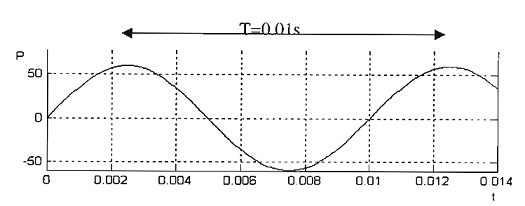
\includegraphics[scale=1]{sinwave}
    \caption{Sóng sin có biên độ 60 dB, tần số 100 Hz}
    \label{fig:c2_sinwave}
\end{figure}

Âm thanh có một số đặc trưng cơ bản như: độ cao, độ mạnh, độ dài và âm sắc.
\begin{itemize}
	\item \textbf{Độ cao} (Pitch): âm thanh luôn có một độ cao nhất định. Độ cao của âm thanh phụ thuộc vào tần số của sóng âm. Tần số càng lớn thì âm thanh càng cao, tần số càng bé thì âm thanh càng trầm.

	\begin{figure}[h]
		\centering
		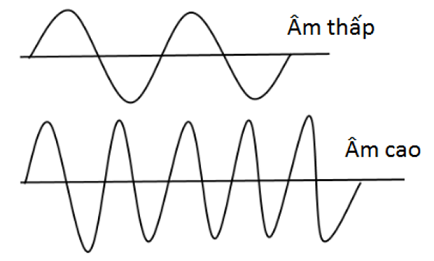
\includegraphics[scale=1]{pitch}
		\caption{Minh họa độ cao (Pitch) của âm}
		\label{fig:c2_pitch}
	\end{figure}

	\item \textbf{Độ mạnh} (Intensity): hay còn gọi là độ to của âm thanh. Độ mạnh của âm thanh phụ thuộc vào biên độ sóng âm. Biên độ càng lớn thi cường độ âm càng mạnh, biên độ càng bé thì cường độ âm càng yếu.
	\item \textbf{Độ dài} (Duration): là thời gian kéo dài của sóng âm.
	\item \textbf{Âm sắc} (Timbre): âm sắc là một đặc trưng sinh lý của âm, giúp phân biết âm thanh do các nguồn khác nhau phát ra. Âm sắc liên quan mật thiết với đồ thị giao động âm.
	\begin{figure}[h]
		\centering
		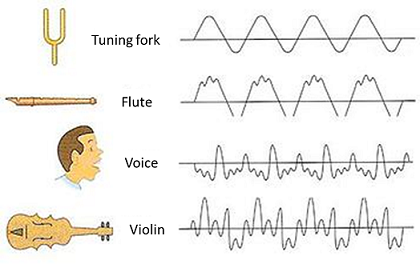
\includegraphics[scale=1]{timbre}
		\caption{Minh họa âm sắc (Timbre) của âm}
		\label{fig:c2_timbre}
	\end{figure}
\end{itemize}

\subsection{Tổng quan về tiếng nói}
Trong tự nhiên, âm thanh bao gồm nhiều loại được tạo ra từ nhiều nguồn khác nhau: 
\begin{itemize}
	\item \textbf{Âm nhạc}: âm thanh được phát ra từ các nhạc cụ.
	\item \textbf{Tiếng kêu}: được phát ra từ các loại động vật. Ví dụ: cá heo (1-164 kHz).
	\item \textbf{Tiếng động}: âm thanh phát ra từ sự va chạm giữa hai vật.
	\item \textbf{Tiếng ồn}: là những âm thanh không mong muốn.
	\item \textbf{Tiếng nói}: là những âm thanh được phát ra từ miệng con người
\end{itemize}

\noindent Ta có thể phân loại tiếng nói dựa theo thanh:
\begin{itemize}
	\item \textbf{Âm hữu thanh}: là âm khi phát ra có sự dao động của đôi dây thanh quản.
	\item \textbf{Âm vô thanh}: phát ra khi đôi dây thanh quản không dao động. Thí dụ phần cuối của phát âm English, chữ sh cho ra âm xát.
\end{itemize}

\noindent Hoặc theo âm:
\begin{itemize}
	\item \textbf{Nguyên âm}: là âm phát ra có thể kéo dài. Tất cả nguyên âm đều là âm hữu thanh, nghĩa là tuần hoàn và khá ổn định trong một đoạn thời gian vài chục ms.
	\item \textbf{Phụ âm}: là âm chỉ phát ra một nhát, không kéo dài được. Có phụ âm hữu thanh và phụ âm vô thanh.
\end{itemize}

Tiếng nói đóng vai trò quan trọng trong hoạt động động giao tiếp giữa con người, nó là phương tiện giao tiếp nhanh, tiện lợi và phổ biến nhất.

\section{Lưu trữ âm thanh trong máy tính}
Tất cả âm thanh mà chúng ta nghe được trong tự nhiên đều tồn tại dưới dạng sóng âm, là các sóng cơ học tuần hoàn liên tục analog. Trong khi đó, máy tính xử lý và lưu trữ thông tin dưới dạng các xung điện tử rời rạc digital. Vì vậy, để có thể lưu trữ và xử lý tín hiệu âm thanh trên máy tính, ta phải mô phỏng sóng âm bằng những mẫu rời rạc. Việc mô phỏng được đặc trưng bởi các thông số:
\begin{itemize}
	\item \textbf{Mẫu (Sample) là gì}: là đơn vị âm thanh nhỏ nhất được lưu trong máy tính. Để có các xung điện tử rời rạc, ta cần lấy mẫu nhiều lần từ tín hiệu analog. Mỗi mẫu là giá trị biên độ của sóng âm tại thời điểm lấy mẫu.
	\item \textbf{Tần số lấy mẫu (Sample Rate)}: là số lần lấy mẫu trên một giây, đơn vị là Hz. Tần số lấy mẫu càng cao, tín hiệu số thu được càng chính xác.
	\item \textbf{Độ dày bit (BitDepth)}: để lưu lại dưới dạng số, mỗi mẫu được biểu diễn bằng một lượng bit dữ liệu nhất định gọi là BitDepth. BitDepth càng lớn âm thanh cáng sắc nét, trung thực.
	\item \textbf{Kênh (Chanel)}: Bằng thuật toán, tín hiệu số có thể được chia thành nhiều kênh để khi nghe bằng hệ thống âm thanh vòm sẽ tạo ra cảm giác thật nhất.
\end{itemize}

Một trong những phương pháp chuyển đổi tín hiệu analog sang digital phổ biến nhất hiện nay là Pulse-Code Modulation (PCM).
Kỹ thuật PCM bao gồm 3 bước:
\begin{itemize}
	\item \textbf{Lấy mẫu (Sampling)}: quá trình rời rạc hoá tín hiệu analog đầu vào theo tần số lấy mẫu f. Ví dụ f = 44100 Hz, ta sẽ lấy mẫu 44100 lần trong một giây.
	\begin{figure}[h]
		\centering
		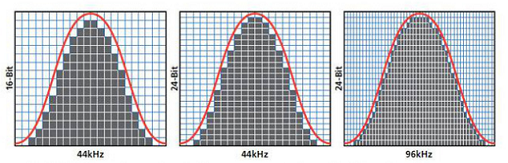
\includegraphics[scale=1]{sampling}
		\caption{Hình minh họa tín hiệu analog được lấy mẫu theo nhiều tần số khác nhau}
		\label{fig:c2_sampling}
	\end{figure}
	\item \textbf{Lượng tử hóa (Quantization)}: tín hiệu analog sau khi được lấy mẫu thì mỗi mẫu có thể có vô số các giá trị. Thay vì sử dụng giá trị mẫu chính xác, giá trị mẫu được thay bằng giá trị gần nhất trong M giá trị cho phép. Các giá trị lượng tử được gọi là các mức lượng tử, nếu các mức lượng tử cách đều nhau gọi là lượng tử đều, ngược lại gọi là lượng tử không đều. Số mức lượng tử M phụ thuộc vào số khả năng mà BitDepth có thể biểu diễn.
	\begin{figure}[h]
		\centering
		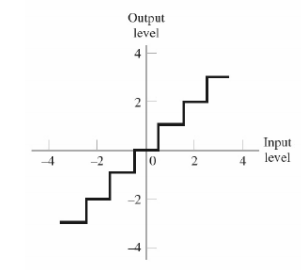
\includegraphics[scale=1]{quantization}
		\caption{Hình minh họa quá trình lượng tử hóa}
		\label{fig:c2_quantization}
	\end{figure}
	\item \textbf{Mã hóa (Encoding)}: Là quá trình biến đổi giá trị các mẫu sau khi lượng tử thành các từ mã dài n bit (n là BitDepth).
\end{itemize}

\begin{figure}[h]
    \centering
    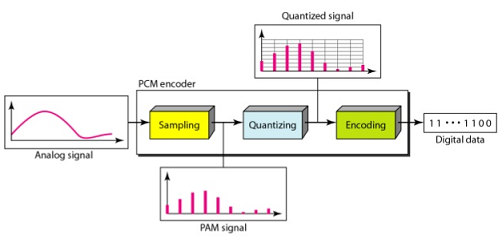
\includegraphics[scale=1]{pcm}
    \caption{Sơ đồ khối mô phỏng phương pháp PCM}
    \label{fig:c2_pcm}
\end{figure}

PCM cùng với những biến thể của nó là nền tảng cho âm thanh số. PCM sẽ sẽ hình thành một dạng sóng, sóng này ít nhiều có thể được chạy ngay bởi một bộ xử lý tín hiệu số. Trong khi hầu hết các định dạng khác khi thao tác với âm thanh thì cần thông qua các thuật toán điều khiển nên phải giải mã chúng khi sử dụng.

\subsection{Lưu trữ không nén (uncompressed)}
Các tín hiệu số thu được thông qua PCM sẽ được lưu trữ nguyên bản, không qua bất kỳ phương pháp nén hay sửa đổi.
\begin{itemize}
	\item \textbf{Ưu điểm}: khi lưu trữ dưới dạng không nén, tín hiệu âm thanh có thể được chạy ngay bởi một bộ xử lý tín hiệu số mà không cần thông qua các thuật toán giải mã.
	\item \textbf{Khuyết điểm}: kích thước tập tin âm thanh sẽ rất lớn làm hao phí không gian lưu trữ và băng thông đường truyền.
\end{itemize}
Các định dạng âm thanh tiêu biểu cho phương pháp lưu trữ không nén là: WAV, AIFF,...

\subsection{Lưu trữ nén}
Các tín hiệu số thu được thông qua PCM sẽ được nén thông qua các thuật toán khác nhau.
\begin{itemize}
	\item \textbf{Ưu điểm}: kích thước tập tin âm thanh nhỏ. Tiết kiệm không gian lưu trữ và băng thông đường truyền.
	\item \textbf{Khuyết điểm}: chất lượng âm thanh có thế bị giảm sút tùy vào thuật toán nén. Tập tin âm thanh muốn thao tác được phải thông qua quá trình giải mã
\end{itemize}

\subsubsection{Nén không mất mát (Lossless compression)}
Các tín hiệu âm thanh gốc sẽ được nén mà không mất dữ liệu và đảm bảo chất lượng ban đầu sau khi giải nén.

Để làm được điều này, cần nhờ đến nhiều thuật toán nén khác nhau. Tuy nhiên, ý tưởng chung của các thuật toán đều là tìm ra quy luật lặp của dữ liệu, sau đó tìm 1 cách hiển thị khác tối ưu hơn, tốn ít dữ liệu hơn. Ví dụ thay vì lưu chuỗi "aaaa bbb cccccc" ta sẽ chuyển thành chuỗi "a4 b3 c6" ít tốn dữ liệu hơn.

Tập tin âm thanh được nén bằng phương pháp này sẽ có tỉ lệ nén không cao, vào khoảng 1/2 đến 1/3 dung lượng âm thanh gốc.

Tiêu biểu cho phương pháp nén không mất mát là các định dạng âm thanh: FLAC, ALAC, APE,...

\subsubsection{Nén có mất mát (Lossy compression)}
Các tín hiệu âm thanh khi được nén sẽ bị loại bỏ đi các thành phần không quan trọng nhằm giảm tối đa kích thước lưu trữ. Mỗi thuật toán nén sẽ có những tiêu chí khác nhau để chọn lựa các thành phần âm thanh sẽ bị bỏ.Ví dụ, ngưỡng nghe của tai người là những âm thanh có tần số từ 14 Hz đến 20 kHz, như vậy thuật toán sẽ bỏ bớt đi các âm thanh có tần số nằm ngoài khoảng đó.

Bên cạnh đó, khi giải mã tập tin âm thanh bị nén, các thuật toán sẽ tạo ra các âm thanh giả nhằm lấp vào các phần đã bị bỏ bớt đi. Hệ quả của việc này là bạn thường nghe các âm thanh méo mó. Các tập tin nhạc được nén với tỉ lệ càng cao thì sự méo tiếng càng nhiều. Bạn sẽ rất dễ dàng nhận ra sự khác biệt khi nghe hai tập tin nhạc gốc và nhạc nén bị mất mát dữ liệu.

Tập tin âm thanh được nén bằng phương pháp này sẽ có tỉ lệ nén rất cao, lên đến 1/10 dung lượng âm thanh gốc.

Tiêu biểu cho phương pháp nén không mất mát là các định dạng âm thanh: MP3, AAC, WMA,...

\section{Ứng dụng}
Hiện nay âm thanh, tiếng nói đã được nghiên cứu và ứng dụng rộng rãi trong nhiều lĩnh vực của cuộc sống như: truyền thông, âm nhạc, chế tạo sonar,...

Trong luận văn này, tiếng nói giữ vai trò quan trọng là phương tiện tương tác chính giữa người dùng và ứng dụng. Người dùng sử dụng tiếng nói để ra lệnh cho ứng dụng, và ứng dụng sử dụng tiếng nói để phản hồi kết quả cho người dùng.

\section{Thư viện PyAudio}
\subsection{Tổng quan}
PyAudio là thư viện mã nguồn mở hỗ trợ người dùng thao tác với âm thanh trên máy tính một cách dễ dàng. PyAudio được viết bằng Python dựa trên thư viện PortAudio. PyAudio có khả năng hoạt động và cài đặt dễ dàng trên đa nền tảng: Windows, Mac OS, và Linux . Tính tới tháng 06/2017 phiên bản mới nhất của PyAudio là 0.2.11

\subsection{Chức năng}
PyAudio cũng cấp tính năng giúp người dùng dễ dàng thu và phát âm thanh từ dữ liệu thô dưới dạng từng sample. PyAudio có thể hoạt động ở chế độ đồng bộ (Synchronous) hoặc không đồng bộ (Asynchronous).

\subsection{Cài đặt}
\begin{itemize}
	\item \textbf{Windows}: python -m pip install pyaudio
	\item \textbf{Mac OS}: brew install portaudio 
pip install pyaudio
	\item \textbf{Linux}: pip install pyaudio
	\item \textbf{Build từ source}: \url{https://people.csail.mit.edu/hubert/git/pyaudio.git}
\end{itemize}

\subsection{Cách sử dụng}
\begin{lstlisting}
"""PyAudio Example: Play a wave file."""
import pyaudio
import wave
import sys
CHUNK = 1024

if len(sys.argv) < 2:
	print("Plays a wave file.\n\nUsage: %s filename.wav" % sys.argv[0])
	sys.exit(-1)

wf = wave.open(sys.argv[1], 'rb')
# instantiate PyAudio (1)
p = pyaudio.PyAudio()
# open stream (2)
stream = p.open(format=p.get_format_from_width(wf.getsampwidth()),
                channels=wf.getnchannels(),
                rate=wf.getframerate(),
                output=True)
# read data
data = wf.readframes(CHUNK)

# play stream (3)
while len(data) > 0:
	stream.write(data)
	data = wf.readframes(CHUNK)

# stop stream (4)
stream.stop_stream()
stream.close()
# close PyAudio (5)
p.terminate()
\end{lstlisting}

Đoạn code trên minh họa cách sử dụng thư viện PyAudio để phát âm thanh từ một file WAV. Chúng tôi sẽ dùng nó để hướng dẫn cách sử dụng đơn giản thư viện PyAudio
\begin{itemize}
	\item Để sử dụng thư viện PyAudio, trước hết cần khởi tạo PyAudio bằng cách sử dụng câu lệnh textbf{pyaudio.PyAudio()} (1). Câu  lệnh này sẽ khởi tạo thư viện PortAudio bên dưới.
	\item Để có thể thu âm hoặc phát audio, ta mở các stream tương ứng bằng câu lệnh \textbf{pyaudio.PyAudio.open()} (2). Input stream để thu âm, output stream để phát audio. Một số tham số cần chú ý trong câu lệnh này:
	\begin{itemize}
		\item \textbf{format}: là định dạng được sử dụng khi encoding. Định dạng này phụ thuộc vào số lượng bit dùng để mã hóa một mẫu (BitDepth).
		\item \textbf{chanels}: số lượng kênh của tập tin âm thanh cần phát hoặc số lượng kênh của âm thanh cần thu âm.
		\item \textbf{rate}: là tần số lấy mẫu (Sample Rate)
		\item \textbf{output}: giá trị này bằng \textbf{true} thì đây là stream output dùng để phát âm thanh.
		\item \textbf{input}: giá trị này bằng \textbf{true} thì đây là stream input dùng để thu âm thanh.
	\end{itemize}
	\item Khi cần phát âm thanh, ta ghi dữ liệu âm thanh lên output stream bằng hàm \textbf{pyaudio.Stream.write()}. Khi cần thu âm thanh, ta đọc dữ liệu âm thanh thu được từ input stream thông qua hàm \textbf{pyaudio.Stream.read()} (3). Đoạn code minh họa đang chạy ở chế độ blocking, nên các hàm \textbf{pyaudio.Stream.write()} và \textbf{pyaudio.Stream.read()} sẽ block chương trình đến khi chúng thực hiện việc đọc/ghi xong.
	\item Để tạm dừng đọc/ghi âm thanh ta dùng hàm \textbf{pyaudio.Stream.stop\_stream()}. Để kết thúc stream ta dùng hàm \textbf{pyaudio.Stream.close()} (4).
	\item Cuối cùng để giải phóng PortAudio ta dùng hàm \textbf{pyaudio.PyAudio.terminate()} (5).
\end{itemize}

\subsection{Các ưu, khuyết điểm}
\begin{itemize}
	\item \textbf{Ưu điểm}: thư viện cài đặt đơn giản, hỗ trợ chạy trên nhiều hệ điều hành.
	\item \textbf{Nhược điểm}: thư viện hỗ trợ ít tính năng. Không hỗ trợ thu âm đồng thời từ nhiều micro.
\end{itemize}

\subsection{Ứng dụng}
Trong luận văn này, thư viên PyAudio đảm nhận vai trò thu âm giọng nói của người dùng. Cung cấp thông tin cho các thành phần khác của hệ thống xử lý.





